\documentclass[aspectratio=169]{beamer}

\usepackage[utf8]{inputenc}
%\usepackage{emoji}

\usepackage{amsmath}
\usepackage{graphicx}
\usepackage[T1]{fontenc}
\usepackage{libertine}
\usepackage{array}
\usepackage{enumitem}
\usepackage{marvosym}

\setitemize{label=\usebeamerfont*{itemize item}%
  \usebeamercolor[fg]{itemize item}
  \usebeamertemplate{itemize item},
}
\setbeamertemplate{itemize item}[square]
\setbeamertemplate{itemize subitem}[circle]

\usepackage{pgfplots}
\usepackage{tikz}
\usetikzlibrary{automata, arrows, positioning, calc, external, babel, backgrounds, matrix, shapes, shadings}
\usepgfplotslibrary{fillbetween}


%%natbib conf
\usepackage[square,authoryear]{natbib}
\renewcommand{\cite}{\citep}
\renewcommand{\bibfont}{\small}
\bibliographystyle{abbrvnat} 


\newcommand{\graphheight}{7cm}
\newcommand{\graphwidth}{11cm}

\newcommand{\E}[1]{E\left[#1 \right]}
\newcommand{\ind}[1]{\mathbf{1}_{#1}}

%\newcommand{\P}[1]{E\left[#1\right]}

% \definecolor{azulcito}{RGB}{20,70,140}
\definecolor{azulcito}{RGB}{0,90,150}
\definecolor{verdecito}{RGB}{90,150,0}
\definecolor{rojito}{RGB}{150,0,90}
\definecolor{violetita}{RGB}{150,20,150}


\setbeamercolor*{structure}{fg=azulcito,bg=azulcito!20!white}
\setbeamercolor*{alerted text}{fg=azulcito}

  \setbeamercolor{block title}{fg=azulcito,bg=azulcito!20!white}
  \setbeamercolor{block body}{fg=black,bg=azulcito!10!white}
  
\beamertemplatenavigationsymbolsempty

\setbeamercolor*{author in head/foot}{fg=azulcito,bg=azulcito!15!white}
\setbeamercolor*{title in head/foot}{fg=azulcito,bg=azulcito!15!white}
\setbeamercolor*{date in head/foot}{fg=azulcito,bg=azulcito!15!white}

% Pgfplots
\pgfplotsset{width=\graphwidth, height = \graphheight, grid style = {dashed, gray}, every tick label/.append style = {font=\footnotesize}, compat=1.18, legend style={font=\footnotesize, draw=none, fill=none}, every axis/.append style={label style={font=\footnotesize}}}

\tikzset{>=stealth}

\newtheorem{proposition}{Proposition}
%\newtheorem{definition}{Definition}
%\newtheorem{lemma}{Lemma}
%\newtheorem{corollary}{Corollary}

\defbeamertemplate*{footline}{mitema}
{
  \leavevmode%
  \hbox{%
  \begin{beamercolorbox}[wd=.25\paperwidth,ht=2.25ex,dp=1ex,left]{author in head/foot}%
    \usebeamerfont{author in head/foot}\hspace*{2ex}\insertshortauthor
  \end{beamercolorbox}%
  \begin{beamercolorbox}[wd=.5\paperwidth,ht=2.25ex,dp=1ex,center]{title in head/foot}%
    \usebeamerfont{date in head/foot}\insertshortdate{}
  \end{beamercolorbox}%
  \begin{beamercolorbox}[wd=.25\paperwidth,ht=2.25ex,dp=1ex,right]{date in head/foot}%
    \insertframenumber{}/\inserttotalframenumber\hspace*{2em} 
  \end{beamercolorbox}}%
 \vskip0pt%
}


\setbeamercolor{blocky}{fg=azulcito,bg=azulcito!15!white}
\setbeamercolor{blocky2}{fg=black,bg=azulcito!10!white}

\defbeamertemplate*{title page}{customized}[1][]
{
{\flushright
  \begin{beamercolorbox}[wd=\paperwidth,sep=1em,right,rightskip=1.5em]{blocky}%
    \usebeamerfont{title}{\huge \inserttitle}\par \bigskip

    \usebeamerfont{subtitle}{\large \insertsubtitle}\par
  \end{beamercolorbox}%
  \vfill
    \usebeamerfont{author}{\Large \insertauthor}\par \vspace{1em}
      \usebeamerfont{institute}{\large \insertinstitute}\par
  
  
  \vfill
  \usebeamerfont{date}{\insertdate}\par
  %\usebeamercolor[fg]{titlegraphic}\inserttitlegraphic
  }
}

\usefonttheme[onlymath]{serif}

\title{Last but not least...}
\subtitle{Matching Earliest-Deadline-First performance through deadline-oblivious policies}

\author[Andres Ferragut, Universidad ORT Uruguay]{Andres Ferragut}
\institute{Universidad ORT Uruguay}
\date[INRIA Paris Seminar -- Jun 2025]{INRIA Paris Seminar -- June 2025}

\AtBeginSection[]
{
\begin{frame}{Outline}
\tableofcontents[currentsection, 
   hideallsubsections, 
   sectionstyle=show/shaded,
]
\end{frame}
}

\newenvironment*{myitem}[1][1.5em]{\begin{itemize}\setlength{\itemsep}{#1}}{\end{itemize}}

\begin{document}

\frame[plain]{\titlepage}

\begin{frame}{Outline}
\tableofcontents
\end{frame}

\section{Introduction}

\begin{frame}{Motivation}{A bit of history...}

	\begin{myitem}
		\item Several queueing systems have service and \alert{timing} requirements.
		\item Examples:
		\begin{itemize}
			\item Computing tasks with real-time constraints.
			\item Item delivery problems in logistics.
			\item Emergency response.
			\item etc. etc. etc.
		\end{itemize}
		\item This has led to a long and rich history of research about \alert{queues with abandonments} \cite{barrer1957queuing,stanford1979reneging,baccellietal1984single}.
	\end{myitem}

\end{frame}

\begin{frame}{Motivation}{Recent developments...}

	One of the most used policies is \alert{Earliest-Deadline-First (EDF)}
	\begin{itemize}
		\item Give priority to tasks with more urgent deadlines.
	\end{itemize}
	\vfill
	\pause
	
	Through fluid limits and diffusion approximations, establish performance:
	\begin{itemize}
		\item \cite{decreusefondmoyal2005fluid} establish EDF fluid limits in the single server case.
		\item \cite{kruketal2011heavy} provides diffusion approximations.
		\item \cite{moyal2013queues} establish some optimality properties of EDF.
		\item \cite{kangramanan2010fluid, kangramanan2012asymptotic} analyze the many-server case.
		\item \cite{ataretal2018law,ataretal2023long} establish asymptotic performance.
	\end{itemize}
	\vfill
	and many others...
\end{frame}

\begin{frame}{Motivation}
	
	\begin{block}{Common assumption}
		\begin{center}
		Customers renege \emph{only} in the queue, and not during service.
		\end{center}
	\end{block}
	\vfill
	\pause

	We call this the \emph{call-center scenario}:

	\begin{itemize}
		\item Akin to waiting for the customer-help line to pick your call while you listen to annoying music.
		
		\item The underlying idea is that when a task reaches service, it will stay until completion.
		
	\end{itemize}
	
	\vfill

	\alert{Key performance metric:} number of satisfied tasks (or reneging probability).

\end{frame}

\begin{frame}{Motivation}{Partial service queues}

	In several queueing systems:

	\begin{itemize}
		\item Tasks may abandon during service.
		\item More importantly, \alert{all service provided may be useful}.
	\end{itemize}

	\vfill

	We call this setting \alert{queues with partial service}.

	\pause

	\vfill

	Some examples:
	\begin{itemize}
		\item Electrical vehicle charging: customers leave the system with a \emph{partial charge}.
		\item LLM inference: longer computation times lead to better answers, but these may be interrupted to deliver a quick response.
		\item File transfers over the Internet, that can be resumed later.
	\end{itemize}

\end{frame}

\begin{frame}{Key points of this talk}
	
	\begin{myitem}
		\item Provide some suitable representation of the state space and dynamics of these partial service queues.
		
		\item Analyze several interesting policies under a suitable fluid model.
		
		\item Compute the main performance metric here: \alert{attained work}.
		
		\item \emph{Last but not least:} show that the simple LCFS policy \alert{exhibits the same performance} than EDF in this setting, without using deadline information. 
	\end{myitem}
\end{frame}

\section{A crash course on measure valued processes}

\begin{frame}{Measure valued stochastic processes}
	
	Consider the simple $M/G/\infty$ queue:
	\begin{itemize}
		\item Tasks arrive as a Poisson process of intensity $\lambda$.
		\item Each task has a service requirement $S\sim g(\sigma)$.
	\end{itemize}
	\vfill
	\begin{center}
		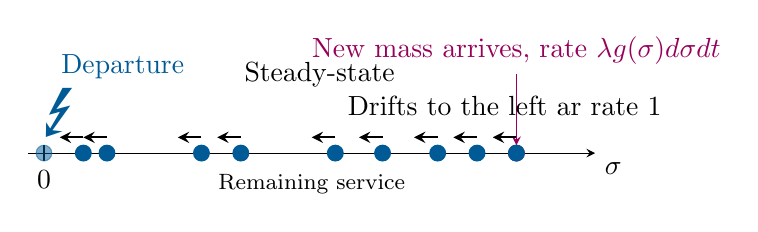
\begin{tikzpicture}    
			\draw [->] (-.2,0) -- node[midway,below,yshift=-1ex]{\footnotesize Remaining service} (7,0);
			\node [below right] at (7,0) {$\sigma$};
			\draw (0,.1) -- (0,-.1) node[below] {$0$};

			\uncover<2>{
				\draw [->,rojito] (6,1) node[above] {New mass arrives, rate $\lambda g(\sigma)d\sigma dt$} -- (6,.1);
				\draw [rojito, fill=rojito] (6,0) circle [radius=0.1];
			}
			\uncover<3>{
				\draw [azulcito, fill=azulcito] (6,0) circle [radius=0.1];
				\draw [thick,->] (6,.2) -- node[midway,above,yshift=1ex] {Drifts to the left ar rate $1$} ++(-.3,0);
			}
			\uncover<4>{
				\draw [azulcito, fill=azulcito, opacity = 0.5, fill opacity=0.5] (0,0) circle [radius=0.1];
				\node[azulcito] at (0.2,0.5) {\Huge\Lightning};
				\node[azulcito] at (1,1.1) {Departure};
			}
			\uncover<5->{
				\foreach \x in {.5,.8,2,2.5,3.7,4.3,5,5.5} {
					\draw [azulcito, fill=azulcito] (\x,0) circle [radius=0.1];
					\draw<5> [thick,->] (\x,.2) --  ++(-.3,0);
				}
				\node at (3.5,1) {Steady-state};
			}

			
		\end{tikzpicture}
	\end{center}
	\vfill
	\uncover<6->{
		\alert{State-descriptor:}
		\begin{equation*}
			\Phi_t = \sum_i \delta_{\sigma_i(t)}
		\end{equation*}
		a Point-process on the positive half-line.
	}
\end{frame}

\begin{frame}{M/G/$\infty$, steady state}
	
	\begin{itemize}
		\item $\Phi_t$ is a measure-valued Markov process.
		\item Its dynamics can be characterized through its generator.
		\item In steady state:
		\begin{equation*}
			\Phi \sim \textrm{Poisson Process with mean measure } \mu(d\sigma) = \lambda \bar{G}(\sigma)d\sigma
		\end{equation*}
		where $\bar{G}$ is the CCDF of $S$.
	\end{itemize}

	\pause
	\vfill
	\alert{Interpretation:}

	\begin{itemize}
	 \item Write $\mu(d\sigma) = \rho \left[\frac{1}{E[S]}(1-G(\sigma))\right]d\sigma$, with $\rho = \lambda E[S]$.
	 \item Then $\left[\frac{1}{E[S]}(1-G(\sigma))\right]d\sigma$ is the \emph{residual service time distribution} associated to $G$.
	 \item In steady-state, the total number of customers $\sim \textrm{Poisson}(\rho)$ and distributed in $\sigma$ as the residual lifetime distribution.
	\end{itemize}

\end{frame}

\begin{frame}{M/G/$\infty$, fluid approximation.}
	
	Suppose that we can replace $\Phi_t$ by a general measure $\mu_t$ with density $f(\sigma;t)$. 
	
	\begin{center}
		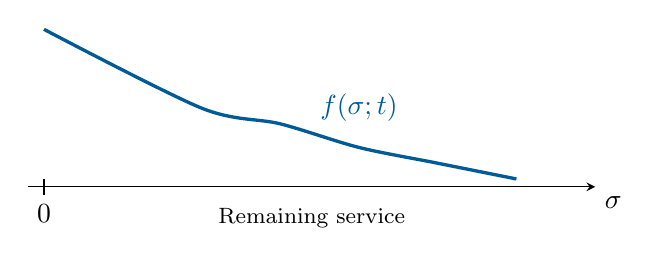
\begin{tikzpicture}    
			\draw [->] (-.2,0) -- node[midway,below,yshift=-1ex]{\footnotesize Remaining service} (7,0);
			\node [below right] at (7,0) {$\sigma$};
			\draw (0,.1) -- (0,-.1) node[below] {$0$};

			\draw [azulcito, very thick] plot [smooth] coordinates {(0,2) (2,1) (3,.8) (4,.5) (5,.3) (6,.1)};
			\node[azulcito] at (4,1) {$f(\sigma;t)$};
		\end{tikzpicture}
	\end{center}
	\begin{itemize}
		\item Mass is transported to the left at rate $1$.
		\item New mass arrives at $\sigma$ with intensity $\lambda g(\sigma)d\sigma dt$.
	\end{itemize}
\vfill
	We can combine this in the following \alert{transport equation}:
	\begin{equation*}
		\frac{\partial f}{\partial t} = \frac{\partial f}{\partial \sigma} + \lambda g(\sigma).
	\end{equation*}

\end{frame}

\begin{frame}{M/G/$\infty$, fluid approximation.}

	Imposing equilibrium and the boundary condition $f(\sigma)\to 0$ as $\sigma\to\infty$ we get:
	\begin{equation*}
		\frac{\partial f}{\partial \sigma} + \lambda g(\sigma) = 0 \Longrightarrow f(\sigma) = \lambda \int_\sigma^{\infty} g(u)\, du = \lambda \bar{G}(\sigma),
	\end{equation*}
	so the fluid approximation recovers the mean measure of $\Phi$.

	\pause\vfill
	\begin{itemize}
		\item This is a deterministic measure, with total mass $\rho$... 
		\item ...distributed in the real line as the residual service distribution.
		\item Serves as an approximation of $\Phi$ in a large scale system ($\lambda\to\infty$).
	\end{itemize}
\end{frame}

\begin{frame}{M/G/$\infty$: take two}{Attained service state descriptor}

	Here is another approach to model the same system \cite{kangramanan2010fluid}:
	\vfill
	\begin{center}
		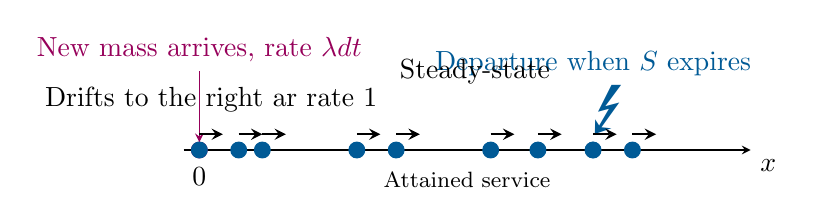
\begin{tikzpicture}    
			\draw [->] (-.2,0) -- node[midway,below,yshift=-1ex]{\footnotesize Attained service} (7,0);
			\node [below right] at (7,0) {$x$};
			\draw (0,.1) -- (0,-.1) node[below] {$0$};

			\uncover<2>{
				\draw [->,rojito] (0,1) node[above] {New mass arrives, rate $\lambda dt$} -- (0,.1);
				\draw [rojito, fill=rojito] (0,0) circle [radius=0.1];
			}
			\uncover<3>{
				\draw [azulcito, fill=azulcito] (0,0) circle [radius=0.1];
				\draw [thick,->] (0,.2) -- node[midway,above,yshift=1ex] {Drifts to the right ar rate $1$} ++(.3,0);
			}
			\uncover<4>{
				\draw [azulcito, fill=azulcito, opacity = 0.5, fill opacity=0.5] (5,0) circle [radius=0.1];
				\node[azulcito] at (5.2,0.5) {\Huge\Lightning};
				\node[azulcito] at (5,1.1) {Departure when $S$ expires};
			}
			\uncover<5->{
				\foreach \x in {.5,.8,2,2.5,3.7,4.3,5,5.5} {
					\draw [azulcito, fill=azulcito] (\x,0) circle [radius=0.1];
					\draw<5> [thick,->] (\x,.2) --  ++(.3,0);
				}
				\node at (3.5,1) {Steady-state};
			}

			
		\end{tikzpicture}
	\end{center}
	\vfill
	\uncover<6->{
		\alert{State-descriptor:}
		\begin{equation*}
			\tilde{\Phi}_t = \sum_i \delta_{x_i(t)}
		\end{equation*}
		a Point-process on the positive half-line, where $x_i(t)$ is the elapsed time in the system
	}

\end{frame}

\begin{frame}{M/G/$\infty$, take two}{Steady-state}
	
	$\tilde\Phi_t$ is a measure-valued Markov process.

	\begin{itemize}
		\item Mass always arrive at $0$ with rate $\lambda dt$.
		\item Transports to the right at rate $1$.
		\item Leaves the system at rate $h(x)$, the \alert{hazard rate function}:
		\begin{equation*}
			h(x) = \lim_{dt\to 0} P(S\in[x,x+dt]\mid S>x) = \frac{g(x)}{\bar{G}(x)} = -\frac{\partial}{\partial x} \log \bar{G}(x).
		\end{equation*}
	\end{itemize}

	\pause
	\vfill
	\alert{Steady-state:}
		\begin{equation*}
			\tilde\Phi \sim \textrm{Poisson Process with mean measure } \nu(dx) = \lambda \bar{G}(x)dx
		\end{equation*}
	
	
	\vfill

	So the reversed representation has the same distribution, because in a random point in time the elapsed service and the remaining service have the same distribution.

\end{frame}


\begin{frame}{M/G/$\infty$: take two}{Fluid approximation.}
	
	Suppose that we can replace $\tilde\Phi_t$ by a general measure $\nu_t$ with density $\tilde f(x;t)$. 
	
	\begin{center}
		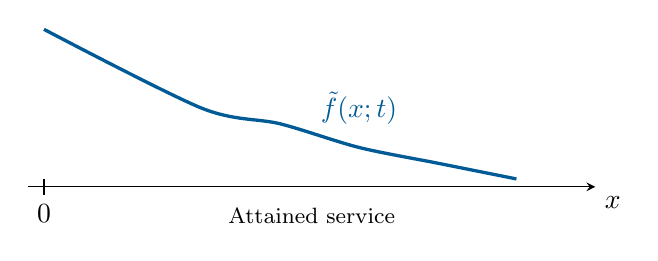
\begin{tikzpicture}    
			\draw [->] (-.2,0) -- node[midway,below,yshift=-1ex]{\footnotesize Attained service} (7,0);
			\node [below right] at (7,0) {$x$};
			\draw (0,.1) -- (0,-.1) node[below] {$0$};

			\draw [azulcito, very thick] plot [smooth] coordinates {(0,2) (2,1) (3,.8) (4,.5) (5,.3) (6,.1)};
			\node[azulcito] at (4,1) {$\tilde f(x;t)$};
		\end{tikzpicture}
	\end{center}
\vfill
\pause
The corresponding transport equation is (informally):
	\begin{equation*}
		\frac{\partial \tilde f}{\partial t} = -\frac{\partial \tilde f}{\partial x} - h(x)\tilde{f} + \lambda \delta_0.
	\end{equation*}
\end{frame}

\begin{frame}{M/G/$\infty$: take two}{Fluid equilibrium.}
	
Imposing equilibrium we get:
	\begin{equation*}
		\frac{\partial \tilde f}{\partial x} = - h(x)\tilde{f} + \lambda \delta_0.
	\end{equation*}

Solving (in a distribution sense) with the boundary condition $\tilde f (\infty) = 0$ we get:
	\begin{equation*}
		\tilde{f}(x) = \lambda e^{-\int_0^x h(u)du}.
	\end{equation*}

But by definition $\int_0^x h(u) du = -\log \bar{G}(x)$, and thus:
	\begin{equation*}
		\tilde{f}(x) = \lambda \bar{G}(x)
	\end{equation*}

So the transport fluid equation recovers again the mean measure of the steady-state.

\end{frame}

\begin{frame}{Lessons learned}

	\begin{myitem}
		\item We can model $M/G$ systems by using two state descriptors:
			\begin{itemize}
				\item The remaining service $\Phi$.
				\item The attained service $\tilde\Phi$.
			\end{itemize}
		\item Both admit reasonable fluid approximations, which correspond to transport equations.
		\item In fact this has been used in the literature to model abandonments (since they operate as $M/G/\infty$ systems in some sense).
	\end{myitem}
	\pause \vfill
	\alert{Question:} can we do more using this machinery of measure-valued processes?
\end{frame}

\section{Partial service queues}

\begin{frame}{Remaining service state descriptor}

  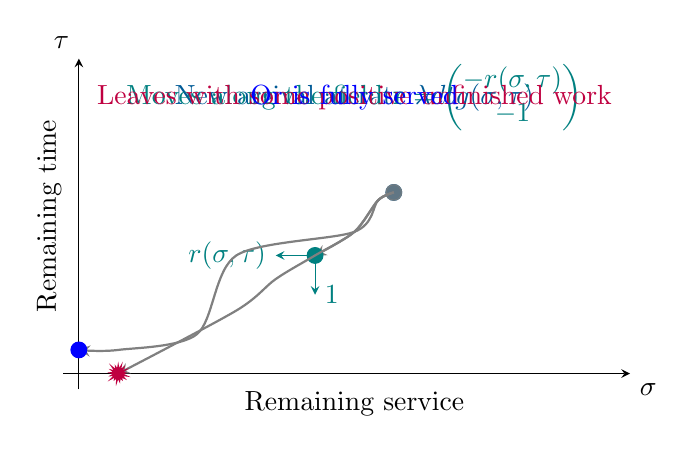
\begin{tikzpicture}
    
  \draw [->] (-.2,0) -- (7,0);
  \node [below right] at (7,0) {$\sigma$};
  \draw [->] (0,-.2) -- (0,4);
  \node [above left] at (0,4) {$\tau$};
  
  \node [below] at (3.5,-.1) {Remaining service};
  \node [rotate=90, left, anchor=south] at (-.1,2) { Remaining time};
  
%	\draw [thick,gray,->] (4,2.3) -- ++(0,-.4);
  \draw<1> [azulcito, fill=azulcito] (4,2.3) circle [radius=0.1];
  \node<1> [azulcito] at (3.5,3.5) {New arrival at rate $\lambda dt g(\sigma,\tau)$};

  \draw<2> [thick,gray,->] plot[smooth] coordinates {(4,2.3) (3.8,2.2) (3.5,1.8) (3,1.5)}; 
  \draw<2> [gray, fill=gray, opacity=0.5] (4,2.3) circle [radius=0.1];
  \draw<2> [teal, fill=teal] (3,1.5) circle [radius=0.1];
  \draw<2> [teal, fill=teal,->] (3,1.5) -- (2.5,1.5) node[left]{$r(\sigma,\tau)$};
  \draw<2> [teal, fill=teal,->] (3,1.5) -- (3,1) node[right]{$1$};
  \node<2> [teal] at (3.5,3.5) {Moves along the field $\mathbf{r} = \begin{pmatrix}
  -r(\sigma,\tau) \\ -1
  \end{pmatrix}$};

  \draw<3> [thick,gray,->] plot[smooth] coordinates {(4,2.3) (3.8,2.2) (3.5,1.8) (3,1.5) (2.5,1.2) (2,.8) (.5,0)}; 
  \draw<3-4> [gray, fill=gray, opacity=0.5] (4,2.3) circle [radius=0.1];
  \node<3>[purple, fill=purple, starburst, inner sep=1.5pt,/pgf/starburst point height=3] at (.5,0) {};
  \node<3> [purple] at (3.5,3.5) {Leaves with some positive unfinished work};

  \draw<4> [thick,gray,->] plot[smooth] coordinates {(4,2.3) (3.8,2.2) (3.5,1.8) (2,1.5) (1.5,.5) (.5,.3) (0,.3)}; 
  \draw<4> [blue, fill=blue] (0,.3) circle [radius=0.1];
  \node<4> [blue] at (3.5,3.5) {Or is fully served};

  \end{tikzpicture}

\end{frame}

\begin{frame}{Example}{Earliest-deadline-first}

  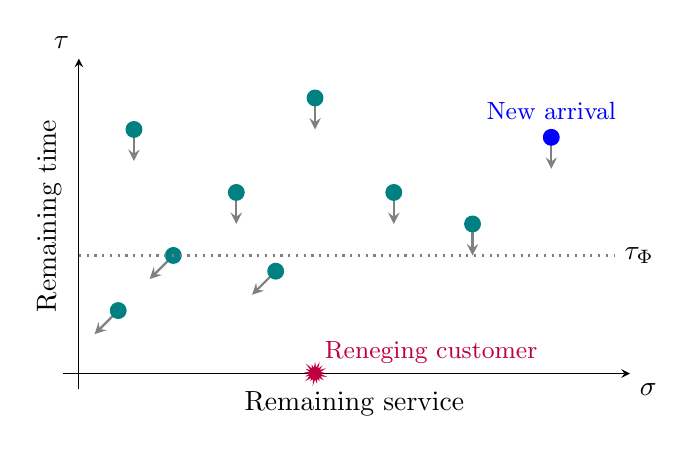
\begin{tikzpicture}
		
	\draw [->] (-.2,0) -- (7,0);
	\node [below right] at (7,0) {$\sigma$};
	\draw [->] (0,-.2) -- (0,4);
	\node [above left] at (0,4) {$\tau$};
	
	\node [below] at (3.5,-.1) {Remaining service};
	\node [rotate=90, left, anchor=south] at (-.1,2) { Remaining time};
	
	\draw [thick,gray,->] (.5,.8) -- ++(-.3,-.3);
	\draw [thick,gray,->] (.7,3.1) -- ++(0,-.4);
	\draw [thick,gray,->] (1.2,1.5) -- ++(-.3,-.3);
	\draw [thick,gray,->] (2,2.3) -- ++(0,-.4);
	\draw [thick,gray,->] (2.5,1.3) -- ++(-.3,-.3);
	\draw [thick,gray,->] (3,3.5) -- ++(0,-.4);
	\draw [thick,gray,->] (4,2.3) -- ++(0,-.4);
	\draw [thick,gray,->] (5,1.9) -- ++(0,-.4);
	\draw [thick,gray,->] (6,3) -- ++(0,-.4);

	\draw [teal, fill=teal] (.5,.8) circle [radius=0.1];
	\draw [teal, fill=teal] (.7,3.1) circle [radius=0.1];
	\draw [teal, fill=teal] (1.2,1.5) circle [radius=0.1];
	\draw [teal, fill=teal]  (2,2.3) circle [radius=0.1];
	\draw [teal, fill=teal] (2.5,1.3) circle [radius=0.1];
	\draw [teal, fill=teal] (3,3.5) circle [radius=0.1];
	\draw [teal, fill=teal] (4,2.3) circle [radius=0.1];
	\draw [teal, fill=teal] (5,1.9) circle [radius=0.1];
	\draw [blue, fill=blue] (6,3) circle [radius=0.1] node[above, yshift=3pt] {\small New arrival};

	%reneging departure
	%\draw [purple, fill=purple!20!white] (3,0) circle [radius=0.1] node[above, anchor=south west] {\small Reneging customer};
	\node[purple, fill=purple, starburst, inner sep=1.5pt,/pgf/starburst point height=3] at (3,0) {};
	\node[purple, anchor=south west] at (3,0){ \small Reneging customer};

	\draw [gray, dotted, thick] (0,1.5) -- (6.8,1.5) node[black, right] {$\tau_\Phi$};

\end{tikzpicture}

\end{frame}

\begin{frame}{Attained service state descriptor}

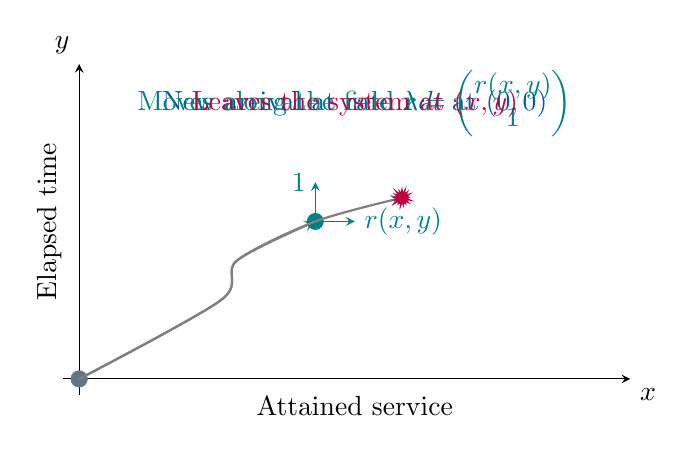
\begin{tikzpicture}
		
	\draw [->] (-.2,0) -- (7,0);
	\node [below right] at (7,0) {$x$};
	\draw [->] (0,-.2) -- (0,4);
	\node [above left] at (0,4) {$y$};
	
	\node [below] at (3.5,-.1) {Attained service};
	\node [rotate=90, left, anchor=south] at (-.1,2) {Elapsed time};

  \draw<1> [azulcito, fill=azulcito] (0,0) circle [radius=0.1];
  \node<1> [azulcito] at (3.5,3.5) {New arrival at rate $\lambda dt$ at $(0,0)$};

  \draw<2> [thick,gray,->] plot[smooth] coordinates {(0,0) (1.8,1) (2,1.5) (3,2)}; 
  \draw<2> [gray, fill=gray, opacity=0.5] (0,0) circle [radius=0.1];
  \draw<2> [teal, fill=teal] (3,2) circle [radius=0.1];
  \draw<2> [teal, fill=teal,->] (3,2) -- (3.5,2) node[right]{$r(x,y)$};
  \draw<2> [teal, fill=teal,->] (3,2) -- (3,2.5) node[left]{$1$};
  \node<2> [teal] at (3.5,3.5) {Moves along the field $\mathbf{r} = \begin{pmatrix}
  r(x,y) \\ 1
  \end{pmatrix}$};

  \draw<3> [thick,gray,->] plot[smooth] coordinates {(0,0) (1.8,1) (2,1.5) (3,2) (4.1,2.3)}; 
  \draw<3> [gray, fill=gray, opacity=0.5] (0,0) circle [radius=0.1];
  \node<3> [purple, fill=purple, starburst, inner sep=1.5pt,/pgf/starburst point height=3] at (4.1,2.3) {};
  \node<3> [purple] at (3.5,3.5) {Leaves the system at $(x,y)$};
\end{tikzpicture}

\end{frame}

\begin{frame}{Example}{Least-Attained-Service policy}
  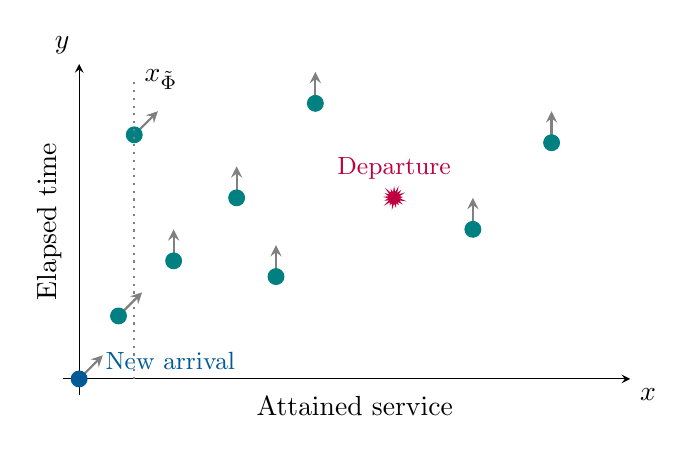
\begin{tikzpicture}
		
	\draw [->] (-.2,0) -- (7,0);
	\node [below right] at (7,0) {$x$};
	\draw [->] (0,-.2) -- (0,4);
	\node [above left] at (0,4) {$y$};
	
	\node [below] at (3.5,-.1) {Attained service};
	\node [rotate=90, left, anchor=south] at (-.1,2) {Elapsed time};
	
	\draw [thick,gray,->] (.5,.8) -- ++(.3,.3);
	\draw [thick,gray,->] (.7,3.1) -- ++(.3,.3);
	\draw [thick,gray,->] (1.2,1.5) -- ++(0,.4);
	\draw [thick,gray,->] (2,2.3) -- ++(0,.4);
	\draw [thick,gray,->] (2.5,1.3) -- ++(0,.4);
	\draw [thick,gray,->] (3,3.5) -- ++(0,.4);
	%\draw [thick,gray,->] (4,2.3) -- ++(.2,.4);
	\draw [thick,gray,->] (5,1.9) -- ++(0,.4);
	\draw [thick,gray,->] (6,3) -- ++(0,.4);

	\draw [teal, fill=teal] (.5,.8) circle [radius=0.1];
	\draw [teal, fill=teal] (.7,3.1) circle [radius=0.1];
	\draw [teal, fill=teal] (1.2,1.5) circle [radius=0.1];
	\draw [teal, fill=teal]  (2,2.3) circle [radius=0.1];
	\draw [teal, fill=teal] (2.5,1.3) circle [radius=0.1];
	\draw [teal, fill=teal] (3,3.5) circle [radius=0.1];
	%\draw [teal!50!white, fill=teal!50!white] (4,2.3) starburst  node[teal,above] {\footnotesize Departure};
	%\node[teal!50!white, fill=teal, starburst, inner sep=1.5pt,/pgf/starburst point height=3] at (4,2.3) {}; 
	%\node[teal,above, yshift=3pt] at (4,2.3) {\footnotesize Departure};
	
    \node[purple, fill=purple, starburst, inner sep=1.5pt,/pgf/starburst point height=3] at (4,2.3) {};
	\node[purple, above, yshift=3pt] at (4,2.3){ \small Departure};
    
    \draw [teal, fill=teal] (5,1.9) circle [radius=0.1];
	\draw [teal, fill=teal] (6,3) circle [radius=0.1];
	
	%new arrival

	\draw [thick,gray,->] (0,0) -- ++(.3,.3);
	\draw [azulcito, fill=azulcito] (0,0) circle [radius=0.1] node[anchor=south west, xshift=6pt] {\small New arrival};
	
	\draw [gray, dotted, thick] (.7,0) -- (.7,3.8) node[black, right] {$x_{\tilde{\Phi}}$};

\end{tikzpicture}

\end{frame}


\begin{frame}{Example}{Last-Come-First-Served policy}
  
  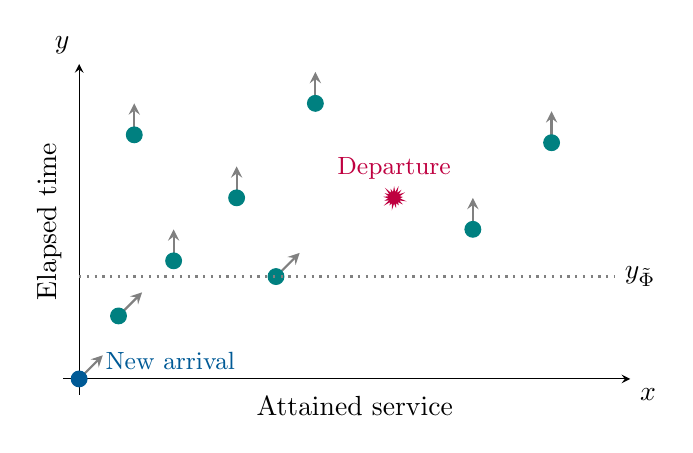
\begin{tikzpicture}
		
	\draw [->] (-.2,0) -- (7,0);
	\node [below right] at (7,0) {$x$};
	\draw [->] (0,-.2) -- (0,4);
	\node [above left] at (0,4) {$y$};
	
	\node [below] at (3.5,-.1) {Attained service};
	\node [rotate=90, left, anchor=south] at (-.1,2) {Elapsed time};
	
	\draw [thick,gray,->] (.5,.8) -- ++(.3,.3);
	\draw [thick,gray,->] (.7,3.1) -- ++(0,.4);
	\draw [thick,gray,->] (1.2,1.5) -- ++(0,.4);
	\draw [thick,gray,->] (2,2.3) -- ++(0,.4);
	\draw [thick,gray,->] (2.5,1.3) -- ++(.3,.3);
	\draw [thick,gray,->] (3,3.5) -- ++(0,.4);
	%\draw [thick,gray,->] (4,2.3) -- ++(.2,.4);
	\draw [thick,gray,->] (5,1.9) -- ++(0,.4);
	\draw [thick,gray,->] (6,3) -- ++(0,.4);

	\draw [teal, fill=teal] (.5,.8) circle [radius=0.1];
	\draw [teal, fill=teal] (.7,3.1) circle [radius=0.1];
	\draw [teal, fill=teal] (1.2,1.5) circle [radius=0.1];
	\draw [teal, fill=teal]  (2,2.3) circle [radius=0.1];
	\draw [teal, fill=teal] (2.5,1.3) circle [radius=0.1];
	\draw [teal, fill=teal] (3,3.5) circle [radius=0.1];
	%\draw [teal!50!white, fill=teal!50!white] (4,2.3) starburst  node[teal,above] {\footnotesize Departure};
	%\node[teal!50!white, fill=teal, starburst, inner sep=1.5pt,/pgf/starburst point height=3] at (4,2.3) {}; 
	%\node[teal,above, yshift=3pt] at (4,2.3) {\footnotesize Departure};
	\draw [teal, fill=teal] (5,1.9) circle [radius=0.1];
	\draw [teal, fill=teal] (6,3) circle [radius=0.1];
			
	\node[purple, fill=purple, starburst, inner sep=1.5pt,/pgf/starburst point height=3] at (4,2.3) {};
	\node[purple, above, yshift=3pt] at (4,2.3){ \small Departure};
	
	%new arrival

	\draw [thick,gray,->] (0,0) -- ++(.3,.3);
	\draw [azulcito, fill=azulcito] (0,0) circle [radius=0.1] node[anchor=south west, xshift=6pt] {\small New arrival};
	
	\draw [gray, dotted, thick] (0,1.3) -- (6.8,1.3) node[black, right] {$y_{\tilde{\Phi}}$};

\end{tikzpicture}

\end{frame}
\begin{frame}{The hazard rate field}

\end{frame}


\section{Performance analysis}

\begin{frame}{Solving the transport equation}{Remaining service case}

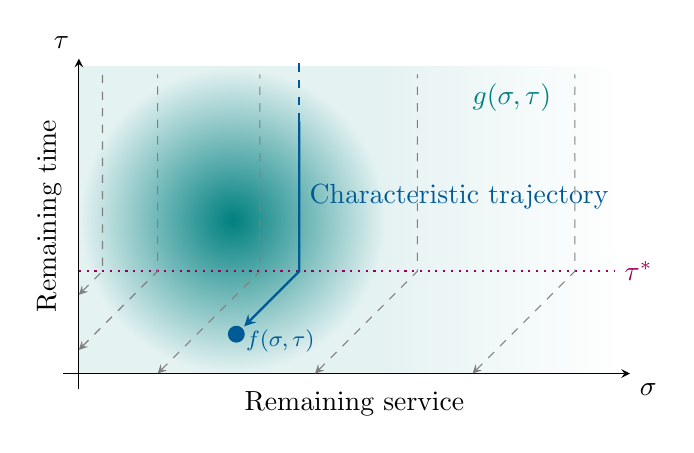
\begin{tikzpicture}
  
	\shade[inner color=teal,outer color=teal!10!white] (0,0) rectangle (3.9,3.9);
	\shade[left color=teal!10!white,right color=white] (3.9,0) rectangle (6.9,3.9);

  \node[teal] at (5.5,3.5) {$g(\sigma,\tau)$};
  \draw [->] (-.2,0) -- (7,0);
  \node [below right] at (7,0) {$\sigma$};
  \draw [->] (0,-.2) -- (0,4);
  \node [above left] at (0,4) {$\tau$};
  
  \node [below] at (3.5,-.1) {Remaining service};
  \node [rotate=90, left, anchor=south] at (-.1,2) {Remaining time};
  
%	\draw [thick,gray,->] (4,2.3) -- ++(0,-.4);
  \draw [rojito, dotted, thick] (0,1.3) -- (6.8,1.3) node[right] {$\tau^*$};
  \draw [azulcito, fill=azulcito] (2,.5) circle [radius=0.1] node[below right, yshift=5pt] {\footnotesize $f(\sigma,\tau)$};

  \draw [azulcito,thick,<-] (2.1,.6) -- (2.8,1.3) -- node[midway, anchor=west] {Characteristic trajectory} (2.8,3.2);
  \draw [azulcito,thick,dashed] (2.8,3.2) -- (2.8,4);

  \draw [gray,dashed,<-] (0,1) -- (.3,1.3) -- (.3,3.8);
  \draw [gray,dashed,<-] (0,.3) -- (1,1.3) -- (1,3.8);
  \draw [gray,dashed,<-] (1,0) -- (2.3,1.3) -- (2.3,3.8);
  \draw [gray,dashed,<-] (3,0) -- (4.3,1.3) -- (4.3,3.8);
  \draw [gray,dashed,<-] (5,0) -- (6.3,1.3) -- (6.3,3.8);

  \end{tikzpicture}

\end{frame}

\begin{frame}{Solving the transport equation}{Attained service case}

	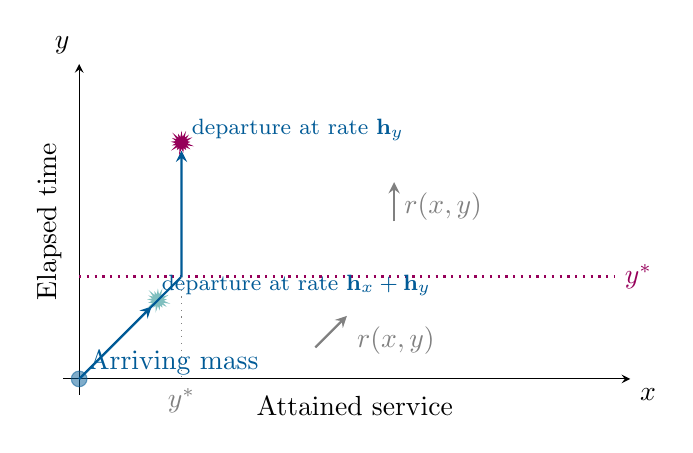
\begin{tikzpicture}
  
		\draw [->] (-.2,0) -- (7,0);
		\node [below right] at (7,0) {$x$};
		\draw [->] (0,-.2) -- (0,4);
		\node [above left] at (0,4) {$y$};
		
		\node [below] at (3.5,-.1) {Attained service};
		\node [rotate=90, left, anchor=south] at (-.1,2) {Elapsed time};

		\draw [gray,thick,->] (3,.4) -- (3.4,.8) node[below right] {$r(x,y)$};
		\draw [gray,thick, ->] (4,2) -- (4,2.5) node[below right] {$r(x,y)$};

		\draw [rojito, dotted, thick] (0,1.3) -- (6.8,1.3) node[right] {$y^*$};
		\draw [azulcito, fill=azulcito, opacity=0.5] (0,0) circle [radius=0.1]; 
		\node<1> [azulcito, anchor=west] at (0,.2) {Arriving mass};
		\draw<2> [azulcito,thick,->] (0,0) -- (.92,.92) node[above right] {\footnotesize departure at rate $\mathbf{h}_x+\mathbf{h}_y$};
		\node<2>[teal!50!white, fill=teal!50!white, starburst, inner sep=1.5pt,/pgf/starburst point height=3] at (1,1) {}; 
		\draw<3> [azulcito,thick,->] (0,0) -- (1.3,1.3) -- (1.3,2.9) node[above right] {\footnotesize departure at rate $\mathbf{h}_y$};
		\node<3>[rojito!50!white, fill=rojito, starburst, inner sep=1.5pt,/pgf/starburst point height=3] at (1.3,3) {}; 
		\draw<3>[gray, dotted] (1.3,1.3) -- (1.3,0) node[below] {$y^*$};

  \end{tikzpicture}


\end{frame}

\begin{frame}{Perceived performance in EDF}
	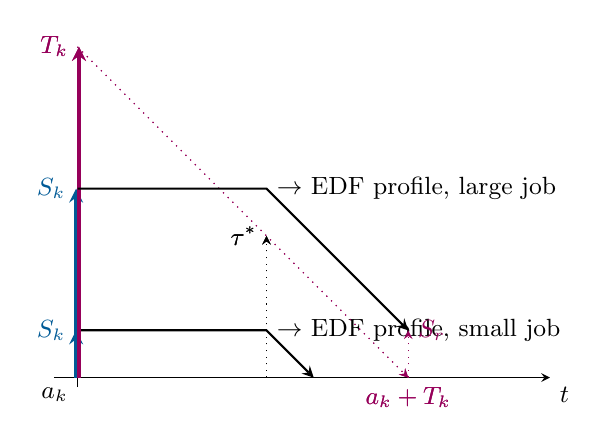
\begin{tikzpicture}[scale=0.6]
			\tikzset{font=\small}
			
			\draw<1-> [->] (-.5,0) -- (10,0);
			\node<1-> [below right] at (10,0) {$t$};
			\draw<1-> [-] (0,-.2) -- (0,.2);
			\node<1-> [below left] at (0,0) {$a_k$};
			
			\draw<1> [very thick,azulcito,->] (-.03,0) -- (-0.03,1) node  [left] {$S_k$};
			\draw<1> [very thick,rojito,->] (.03,0) -- (0.03,7) node  [left] {$T_k$};
			\draw<1> [dotted,rojito,->] (0,7) -- (7,0) node [below] {$a_k+T_k$};
			\draw<1> [black,thick,->] (0,1) -- (4,1) node [ right] {\small $\to$ EDF profile, small job}  --  (5,0);
			\draw<1> [black,dotted,->] (4,0) -- (4,3) node [left] {$\tau^*$};
			
			\draw<2-> [very thick,azulcito,->] (-.03,0) -- (-0.03,4) node  [left] {$S_k$};
			\draw<2-> [very thick,rojito,->] (.03,0) -- (0.03,7) node  [left] {$T_k$};
			\draw<2-> [dotted,rojito,->] (0,7) -- (7,0) node [below] {$a_k+T_k$};
			\draw<2-> [black,thick,->] (0,4) -- (4,4)  node [ right] {\small $\to$ EDF profile, large job} -- (7,1);
			\draw<2-> [black,dotted,->] (4,0) -- (4,3) node [left] {$\tau^*$};
			\draw<2-> [rojito,dotted,->] (7,0) -- (7,1) node [right] {$S_r$};
			
	\end{tikzpicture}
\end{frame}

\begin{frame}{Perceived performance in LAS and LCFS}
	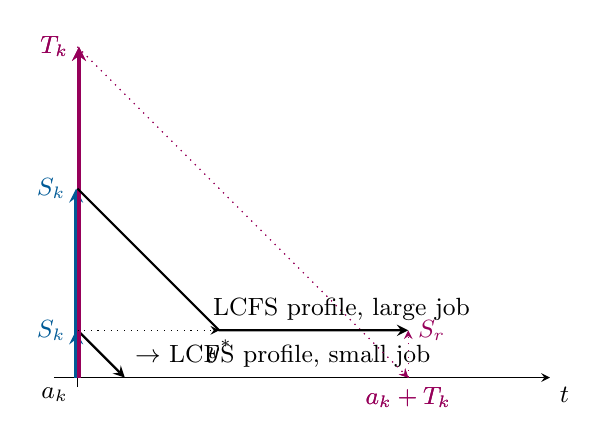
\begin{tikzpicture}[scale=0.6]
			\tikzset{font=\small}
			
			\draw<1-> [->] (-.5,0) -- (10,0);
			\node<1-> [below right] at (10,0) {$t$};
			\draw<1-> [-] (0,-.2) -- (0,.2);
			\node<1-> [below left] at (0,0) {$a_k$};
			
			\draw<1> [very thick,azulcito,->] (-.03,0) -- (-0.03,1) node  [left] {$S_k$};
			\draw<1> [very thick,rojito,->] (.03,0) -- (0.03,7) node  [left] {$T_k$};
			\draw<1> [dotted,rojito,->] (0,7) -- (7,0) node [below] {$a_k+T_k$};
			\draw<1> [black,thick,->] (0,1) -- (1,0) node [above right] {\small $\to$ LCFS profile, small job};
			
			\draw<2-> [very thick,azulcito,->] (-.03,0) -- (-0.03,4) node  [left] {$S_k$};
			\draw<2-> [very thick,rojito,->] (.03,0) -- (0.03,7) node  [left] {$T_k$};
			\draw<2-> [dotted,rojito,->] (0,7) -- (7,0) node [below] {$a_k+T_k$};
			\draw<2-> [black,thick,->] (0,4) -- (3,1) -- node [above, xshift=10pt] {\small LCFS profile, large job} (7,1);
			\draw<2-> [black,dotted,->] (0,1) -- (3,1) node [below] {$y^*$};
			\draw<2-> [rojito,dotted,->] (7,0) -- (7,1) node [right] {$S_r$};
			
	\end{tikzpicture}
\end{frame}

\section{Simulations}


\section{Future work}

\begin{frame}{Final remarks}
	
\end{frame}


\begin{frame}[plain]
	\vfill
	{\Huge \alert{Merci beaucoup!}}
	\vfill
	Andres Ferragut

	\smallskip

	\href{mailto://ferragut@ort.edu.uy}{\alert{ferragut@ort.edu.uy}}
	
	\smallskip

	\href{http://aferragu.github.io}{\alert{https://aferragu.github.io}}
\end{frame}

\begin{frame}[allowframebreaks]{References}
	\bibliography{reneging}
\end{frame}
\end{document}
